\chapter{Un esame di laboratorio risolto}
Questa appendice l'ho realizzata per dare un'idea di come andrebbe scritto un codice in linea con le richieste di Informatica 1. Ho cercato di usare lo stile e gli strumenti più semplici possibili: il minimo richiesto per superare l'esame a pieni voti! 
Volendo si possono usare tanti altri strumenti: classi, template, ecc ecc... Ma se sai queste cose, guardare questo svolgimento per te è probabilmente inutile!
A proposito del ``tutto giusto'': mi sono concentrato sul codice, per quanto riguarda la correttezza dei risultati\ldots non assicuro nulla!


Cos'è apprezzato nell'esame di Informatica 1, ovvero cosa devi fare per prendere un bel voto?
\begin{itemize}
\item I risultati devono essere corretti (ma questo è ovvio\ldots).
\item Il codice deve essere comprensibile e leggibile; potrà sembrarti una cavolata, ma ad ogni parentesi graffa dopo dai i dovuti spazi di tab per renderlo ordinato!
\item Il codice deve essere ben strutturato: devi scrivere il meno possibile nel main, dove invece dovresti limitarti a poco più di semplici chiamate a funzione. Ogni volta che puoi, e che ha senso farlo, scrivi una funzione che esegua un'insieme di operazioni.
\item Dividi il codice in librerie: le funzioni non tenerle nello stesso file del main, ma crea una, o piu', librerie. 
\item Scrivi un makefile ben fatto e funzionante.
\item Stai attento a quelli che possono sembrarti dettagli ma che sono importanti in un buon codice: ogni volta che apri uno stream ad un file controlla che non sia corrotto ma che sia funzionante; quando non ti serve più lo stream ricordati di chiuderlo e di non lasciarne nessuno in sospeso; dopo che hai allocato la memoria, quando non serve più, liberala! 
\item Sicuramente apprezzato: nei passaggi oscuri, commenta un minimo il codice per semplificarne la lettura, potrebbe aiutare il professore a capire cosa avevi in mente.
\end{itemize}



Un consiglio: se non sei molto pratico, durante l'esame ogni volta che scrivi un pezzo di codice compilalo e provalo. Non cercare di scrivere tutto e solo alla fine provare a compilare: è praticamente impossibile scrivere tanto codice senza fare neanche un piccolo errore. Trovare un errore in un pezzetto di codice è più facile che capire perché un intero programma non funziona. 

Procedi per piccoli passi: scrivi una funzione (tipo carica da file) e testala, se è corretta salva tutto e vai avanti. Se ad un certo punto si romperà tutto --in stile segmentation fault o cose strane-- saprai che al passo precedente funzionava tutto e ti basterà tornare indietro o aggiustare il nuovo pezzo di codice. 

Non c'è nulla di peggio di scrivere l'intero programma, testarlo per la prima volta dieci minuti prima della consegna e ritrovarsi come output un segmentation violation.

E, soprattutto, meglio un programma non completo (ma che compila) di uno finito ma che non compila (rischio bocciatura!)!
\newpage
\section{21 Luglio 2015}
Il testo è il seguente:\\
\begin{figure}[ht] 
	\centering
%	\includepdf[scale=0.8,pages=2-,frame]{#1}
	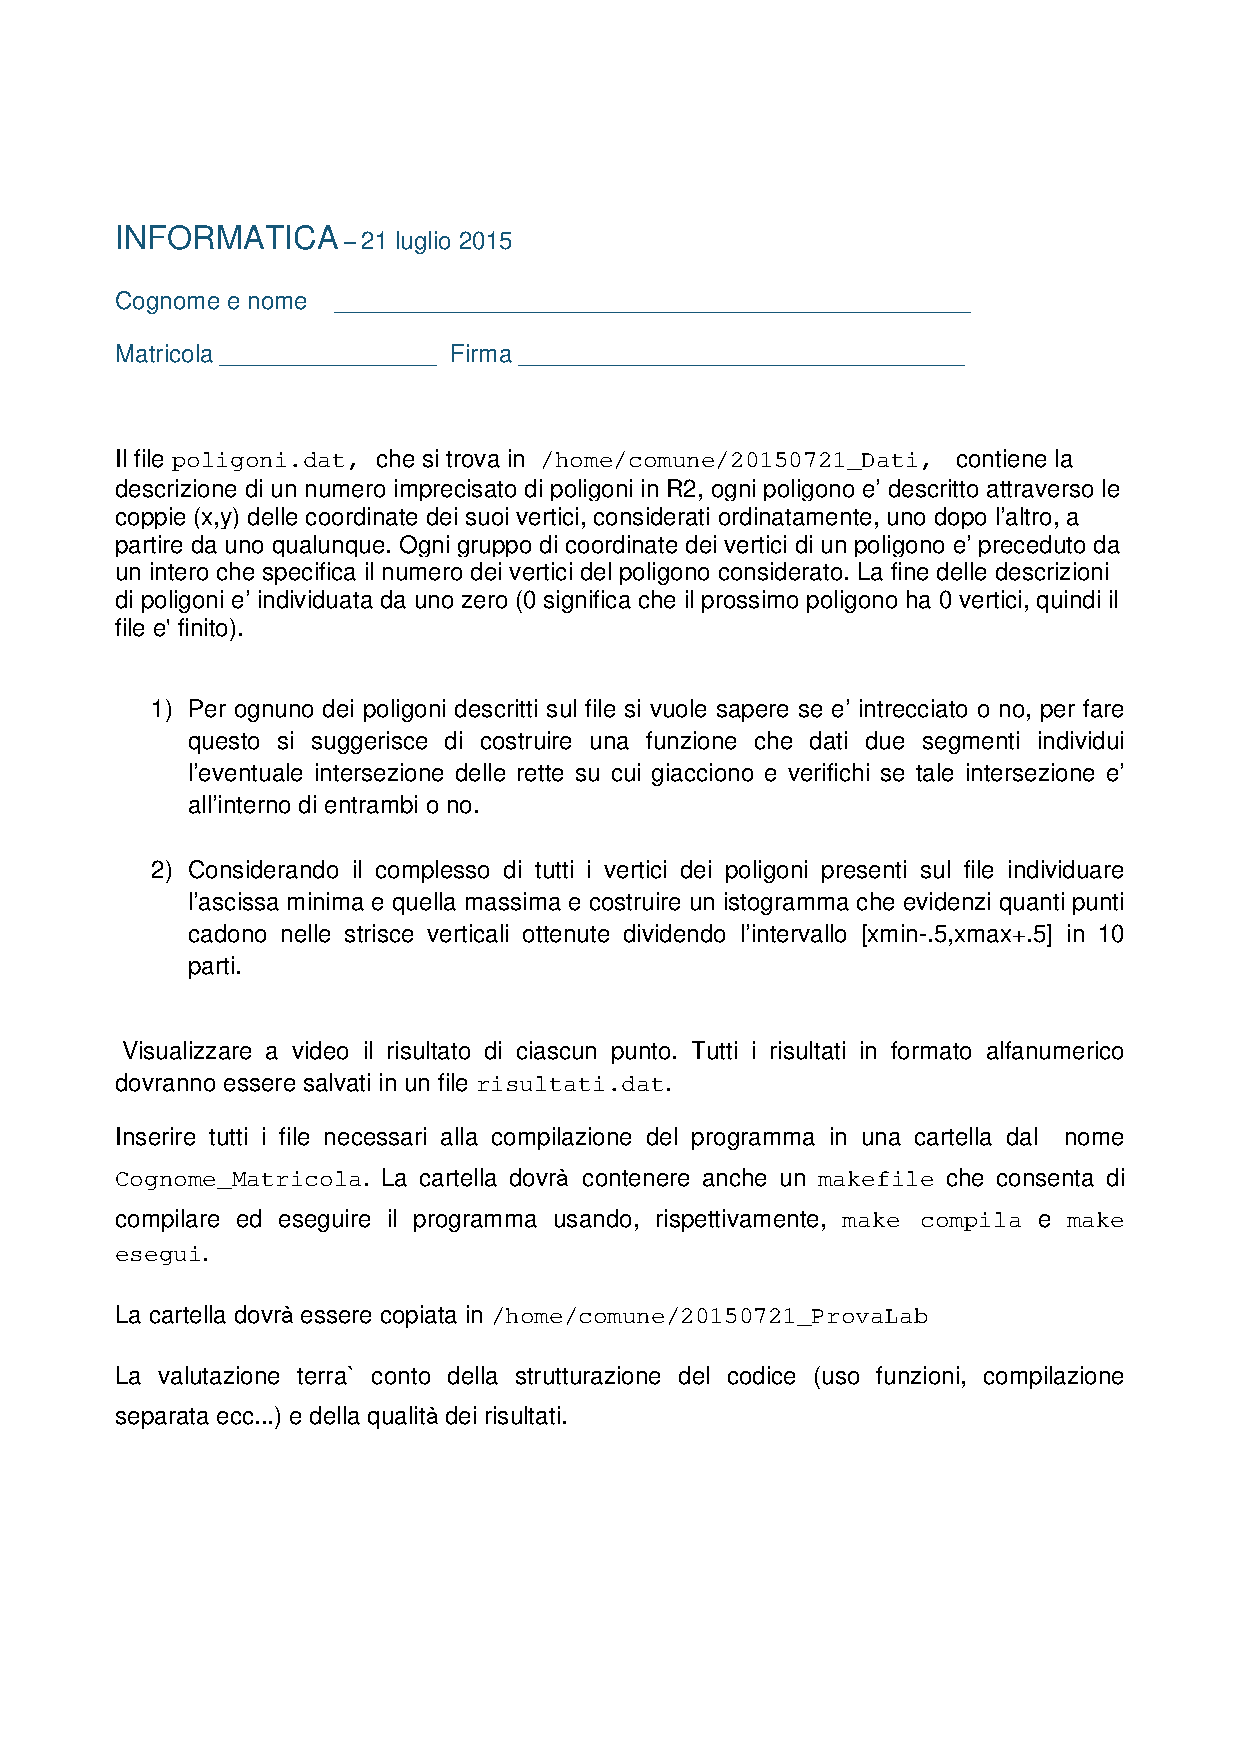
\includepdf[scale=0.88,pages=1]{esami/Esame210715/testo.pdf}
	%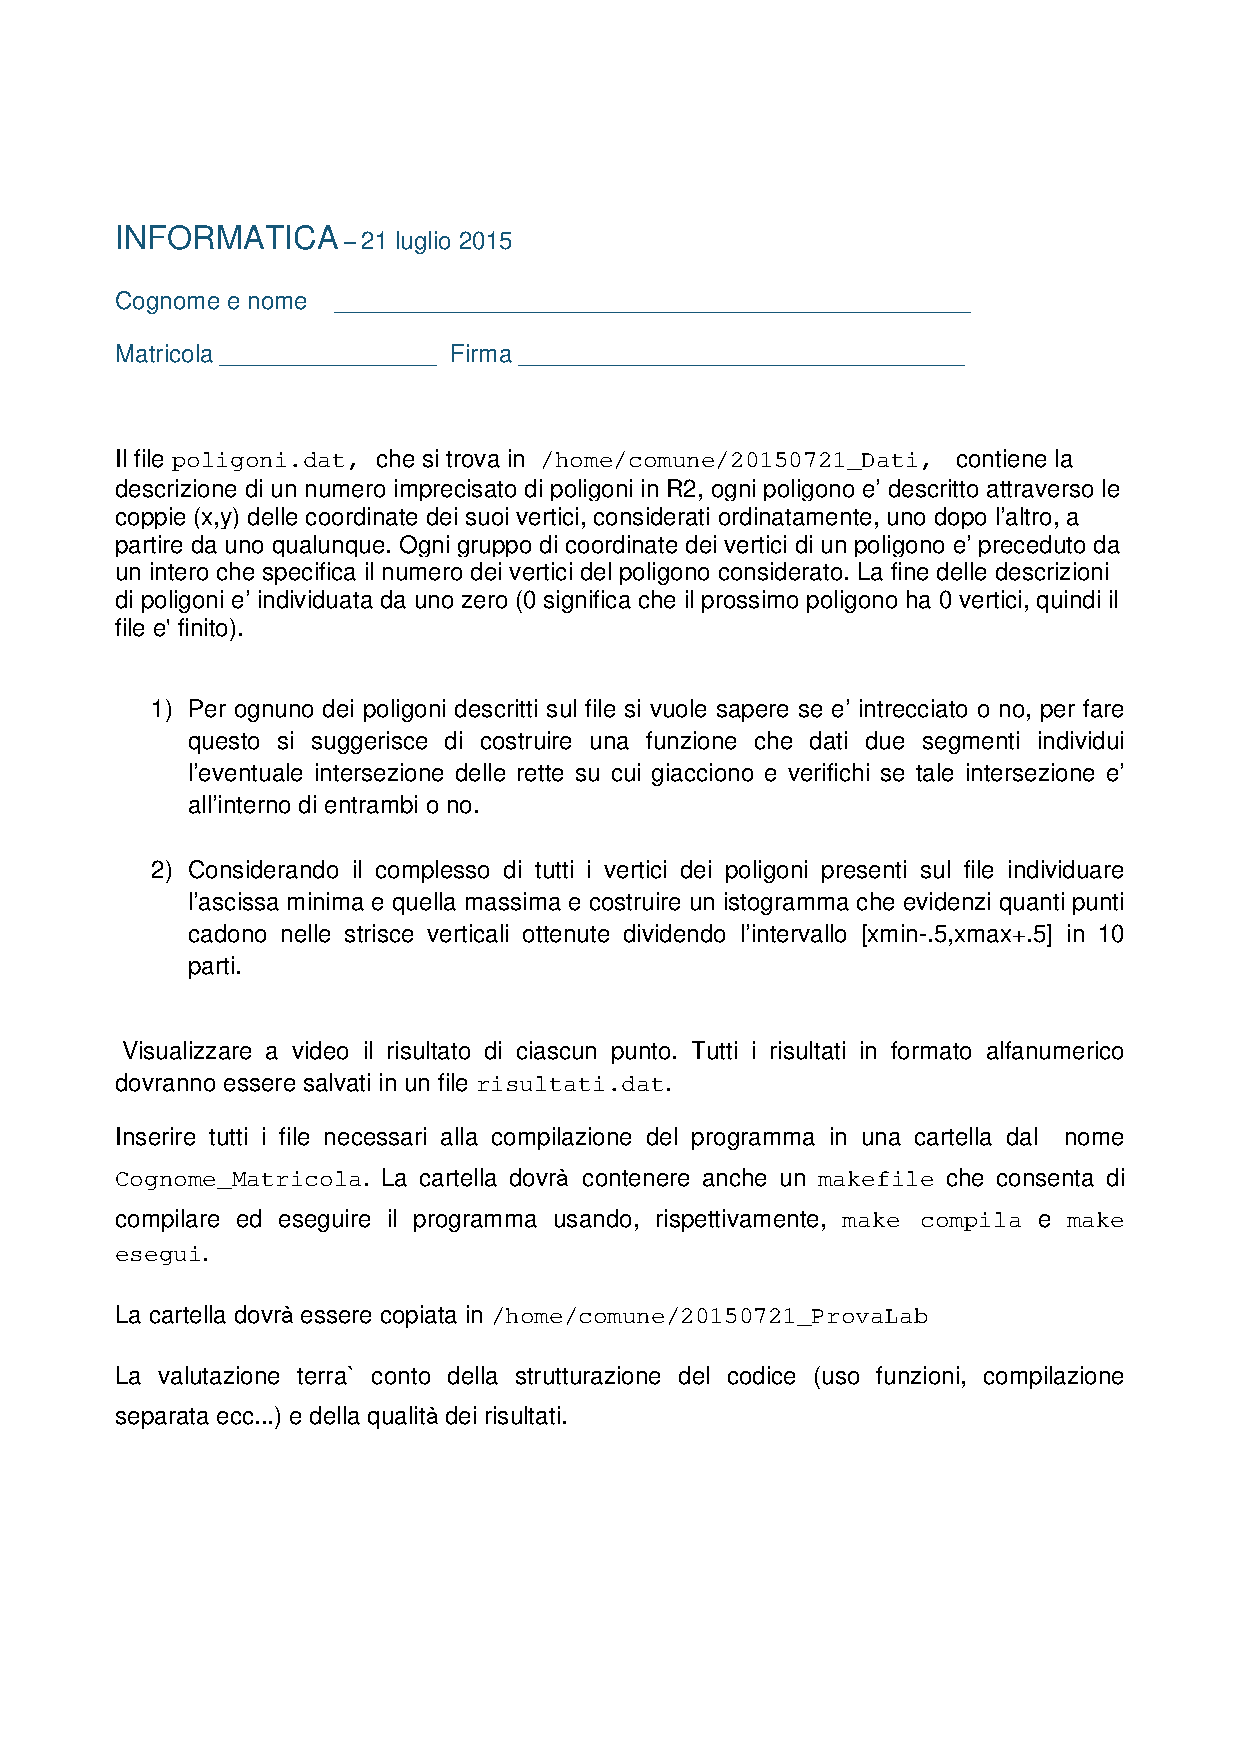
\includegraphics[scale=0.55]{esami/Esame210715/testo.pdf}
%	\caption{Testo dell'esame}
\end{figure}  
\newpage

Il nostro codice è diviso in:  \verb|makefile|, \verb|main.cpp|, \verb|funzioni.h|, \verb|funzioni.cpp|; ti riporto anche \verb|poligoni.dat| se vuoi provare sui dati dell'esame.
\subsection*{makefile}
\lstinputlisting[language=make]{esami/Esame210715/makefile}
\subsection*{main.cpp}
\lstinputlisting{esami/Esame210715/main.cpp}
\subsection*{funzioni.h}
\lstinputlisting{esami/Esame210715/funzioni.h}
\subsection*{funzioni.cpp}
\lstinputlisting{esami/Esame210715/funzioni.cpp} %TODO rimuovere appo!!!
\subsection*{poligoni.dat}
\lstinputlisting{esami/Esame210715/poligoni.dat}
